\documentclass{article}

\usepackage{graphicx}
\usepackage{tikz}
\usepackage{tikzsymbols}
\usetikzlibrary{calc,patterns,shapes.geometric}
\pagestyle{empty}
\usepackage[margin=0pt]{geometry}
\geometry{papersize={14in,12in}}

\def\centerarc[#1](#2)(#3:#4:#5){\draw[#1] ($(#2)+({#5*cos(#3)},{#5*sin(#3)})$) arc (#3:#4:#5);}

\begin{document}
	\begin{figure}
		\centering
		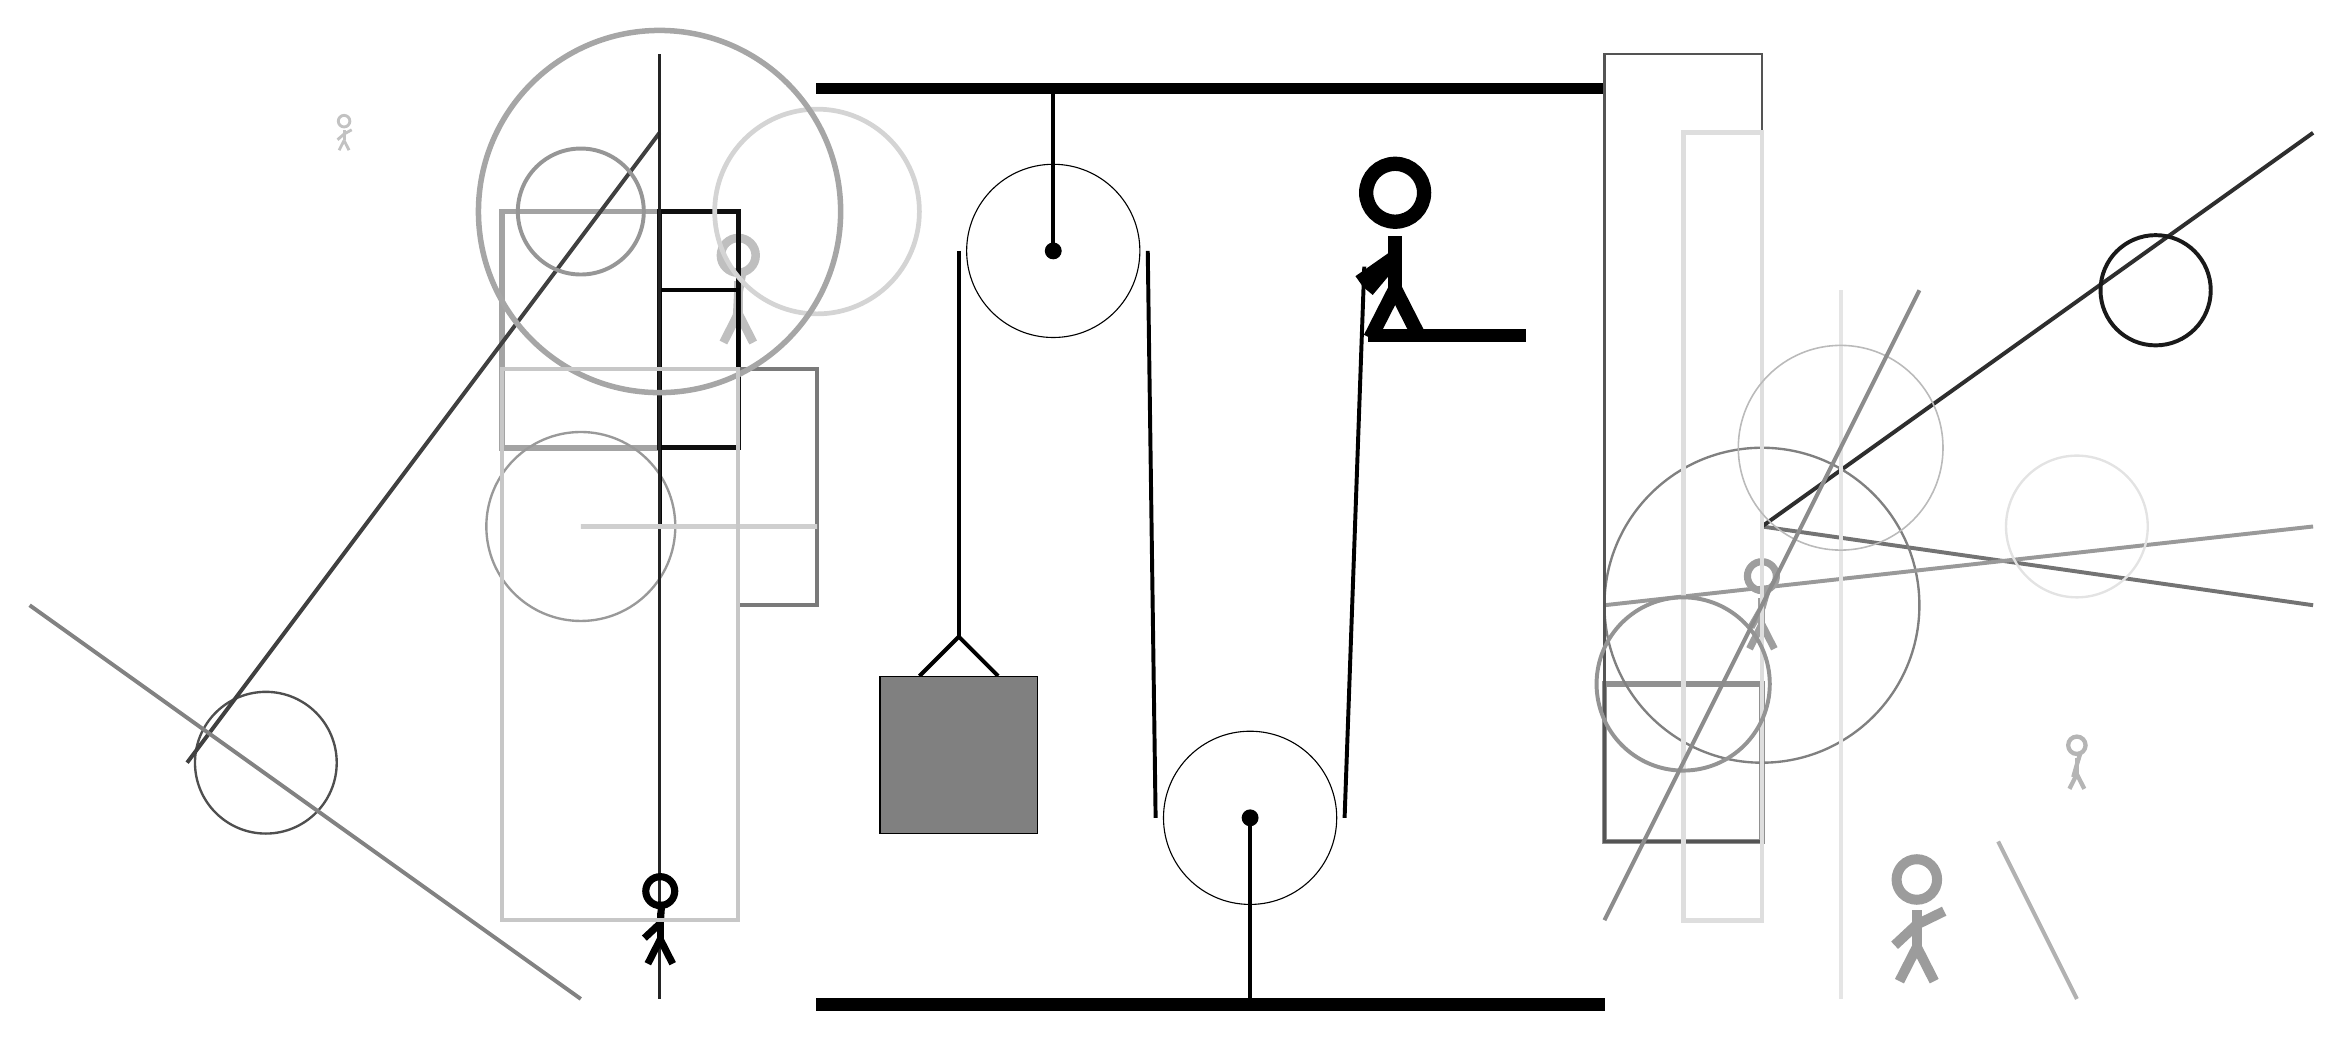
\begin{tikzpicture}
			%%%%% START %%%%%
			
			\draw[fill=black] (-2, 11.5) rectangle (8, 11.625);
			
			\draw (3.5, 2.3) circle (1.1);
			\draw[fill=black] (3.5, 2.3) circle (0.1);
			\draw[line width=0.5mm] (3.5, 2.3) -- (3.5, 0);
			
			\draw (1, 9.5) circle (1.1);
			\draw[fill=black] (1, 9.5) circle (0.1);
			\draw[line width=0.5mm] (1, 11.5) -- (1, 9.5);
			
			\draw[line width=0.5mm](-0.7, 4.1) --  (-0.2, 4.6) -- (0.3, 4.1);
			\draw[fill=black!50] (-1.2, 4.1) rectangle (0.8, 2.1);
			
			\draw[line width=0.5mm](-0.2, 9.5) -- (-0.2, 4.6);
			\centerarc[line width=0.5mm](1, 9.5)(180:0:1.2000000000000002)
			\draw[line width=0.5mm](2.2, 9.5) -- (2.3, 2.3);
			\centerarc[line width=0.5mm](3.5, 2.3)(180:360:1.2000000000000002)
			\draw[line width=0.5mm](4.7, 2.3) -- (4.95, 9.3);
			
			\draw[line width=0.5mm, color=black!55](10, 6) -- (17, 5);
			
			\draw[line width=0.7mm, color=black!43] (10, 2) rectangle (8, 4);
			\node[line width=0.2mm, color=black!25] at (-3, 9) {\Strichmaxerl[6][87][80]};
			\node[line width=0.6mm, color=black!24] at (-8, 11) {\Strichmaxerl[2][41][29]};
			\draw[line width=0.5mm, color=black!82](10, 6) -- (17, 11);
			
			\draw[line width=0.7mm, color=black!36] (-4, 7) rectangle (-6, 10);
			\draw [line width=0.3mm, color=black!40](-5, 6) circle (1.2);
			
			\draw [line width=0.3mm, color=black!69](-9, 3) circle (0.9);
			\draw[line width=0.6mm, color=black!94] (-4, 10) rectangle (-3, 7);
			\draw[line width=0.5mm, color=black!98] (-3, 6) rectangle (-4, 9);
			\draw[line width=0.5mm, color=black!52] (-2, 5) rectangle (-3, 8);
			
			\draw [line width=0.6mm, color=black!17](-2, 10) circle (1.3);
			\draw[line width=0.5mm, color=black!75](-4, 11) -- (-10, 3);
			\draw [line width=0.3mm, color=black!50](10, 5) circle (2.0);
			\draw[line width=0.5mm, color=black!40](8, 5) -- (17, 6);
			\draw[line width=0.3mm, color=black!67] (8, 2) rectangle (10, 12);
			
			\draw[line width=0.5mm, color=black!30](13, 2) -- (14, 0);
			\draw [line width=0.5mm, color=black!41](-5, 10) circle (0.8);
			\node[line width=0.6mm, color=black!38] at (10, 5) {\Strichmaxerl[5][60][74]};
			
			\node[line width=0.7mm, color=black!39] at (12, 1) {\Strichmaxerl[7][43][26]};
			\draw [line width=0.3mm, color=black!11](14, 6) circle (0.9);
			
			\draw[line width=0.4mm, color=black!86] (-4, 12) rectangle (-4, 0);
			\draw[line width=0.4mm, color=black!20] (-3, 5) rectangle (-3, 1);
			\draw[line width=0.7mm, color=black!19] (-2, 6) rectangle (-5, 6);
			\node[line width=0.3mm, color=black!100] at (-4, 1) {\Strichmaxerl[5][43][86]};
			
			\draw[line width=0.6mm, color=black!13] (9, 11) rectangle (10, 1);
			\draw [line width=0.7mm, color=black!35](-4, 10) circle (2.3);
			\draw [line width=0.5mm, color=black!42](9, 4) circle (1.1);
			
			\node[line width=0.2mm, color=black!29] at (14, 3) {\Strichmaxerl[3][74][73]};
			\draw[line width=0.5mm, color=black!10](11, 0) -- (11, 9);
			\draw [line width=0.2mm, color=black!27](11, 7) circle (1.3);
			
			\draw[line width=0.5mm, color=black!49](-5, 0) -- (-12, 5);
			\draw[line width=0.5mm, color=black!45](8, 1) -- (12, 9);
			
			\draw [line width=0.5mm, color=black!90](15, 9) circle (0.7);
			\draw[line width=0.5mm, color=black!22] (-3, 8) rectangle (-6, 1);
			
			\node at (5.3, 9.5) {\Strichmaxerl[10][35][-130]};
			\draw[fill=black] (5, 8.5) rectangle (7, 8.35);
			
			\draw[fill=black] (-2, 0) rectangle (8, -0.15);
			
			%%%%% END %%%%%
		\end{tikzpicture}
	\end{figure}	
\end{document}